\documentclass[tikz,border=8pt]{standalone}
\usepackage[UTF8,fontset=fandol]{ctex}
\usepackage{amsmath,amssymb,bm}
\usetikzlibrary{arrows.meta,calc,decorations.pathmorphing}
\tikzset{arr/.style={-{Stealth[length=2mm]},semithick},
dot/.style={circle,fill,inner sep=1.5pt}}
\begin{document}
\small

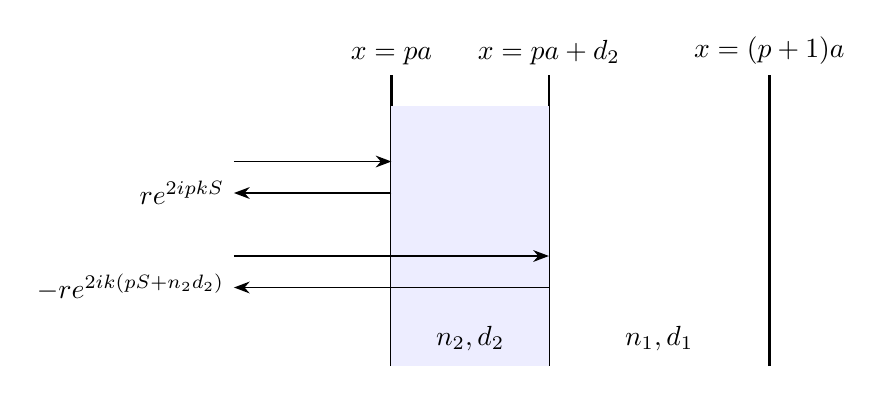
\begin{tikzpicture}
\draw[thick] (0,-1.5)--(0,2.2) node[above] {$x=pa$};
\draw[thick] (2,-1.5)--(2,2.2) node[above] {$x=pa+d_2$};
\draw[thick] (4.8,-1.5)--(4.8,2.2) node[above] {$x=(p+1)a$};
\fill[blue!7] (0,-1.5) rectangle (2,1.8);
\node at (1,-1.15) {$n_2,d_2$};
\node at (3.4,-1.15) {$n_1,d_1$};
\draw[arr] (-2,1.1)--(0,1.1);
\draw[arr] (0,.7)--(-2,.7);
\draw[arr] (-2,-.1)--(2,-.1);
\draw[arr] (2,-.5)--(-2,-.5);
\node[left] at (-2,.7) {$r e^{2ipkS}$};
\node[left] at (-2,-.5) {$-r e^{2ik(pS+n_2d_2)}$};
\end{tikzpicture}
\end{document}
